%!TEX root = vmf_main.tex

\section{Format Definition}

VMF is built on top of the JSON format for two principal reasons. Firstly, VMF is composed primarily of ordered collections of integers for time and pitch data along with a header composed of key-value pairs. Because the VMF's representation only requires these two types of data structures, JSON is a perfect fit as JSON arrays provide an ordered collection, and JSON objects provide a collection of key-value pairs. Secondly, because JSON is an extremely popular data format, compatible tools and other parsers are readily available in many different programming languages for consuming the VMF format.

Before describing the format in detail, Figure \ref{fig:completeExample} displays a complete example which can be referenced during the following discussion.

\begin{figure}
  \begin{center}
    \begin{Verbatim}[fontfamily=courier, xleftmargin=\parindent]
    {
      "header": {
        "tick_value": "1",
        "number_of_parts": 2,
        "number_of_voices": 2,
        "time_signature": {
            "0.0": "2/4"
        },
        "key_signature": {
            "0.0": 0
        },
        "tempo": {
          "0.0": 100
        }
      },
      "body": [
        [[1,-1,0,0,4,0],[1,-1,0,0,4,1]],
        [[1,-1,0,4,4,0],[2,-1,0,0,4,1]],

        [[1,-1,0,7,4,0],[1,-1,0,7,4,1]],
        [[1,-1,0,4,4,0],[2,-1,0,7,4,1]]
      ]
    }
    \end{Verbatim}
    \caption{Complete VMF example of a two part score}
    \label{fig:completeExample}
  \end{center}
\end{figure}

\subsection{VMF Header}

In order to interpret the musical data contained in a VMF file, some global information is required for reference. In VMF, this information is stored in the file header. The header object is a JSON object containing information regarding the score's structure, global musical signatures, and the sampling rate produced by the vectors in the body.

\subsubsection{Voices and Parts}

The first two header paramters of importance are ``number\_of\_parts'' and ``number\_of\_voices''. A VMF file is divided into several musical parts which each represent the music played by a single instrument or section. A part is then further subdivided into 1 or more voices. This would cover the case where an instrument is capable of playing more than one melodic line simultaneously such as the guitar or the piano.

The number of parts can be calculated by simply counting the number of individual parts contained in a score. The number of voices in a score is calculated a little bit differently; the maximum number of simultaneous voices in each part must be determined and these maximum values must be added together to arrive at the final value.

For example, when examining Figure \ref{fig:voicesExample}, it is clear that there are four distinct parts (soprano, alto, tenor and bass), and therefore the number of parts recorded in the header would be four. Upon further examination, it can be seen that the soprano, alto and bass parts each have a maximum of 1 voice, while the tenor part has a maximum of 2 voices (measures 1-3). Because of this, the total number of voices in this example is five (the sum of the maximm number of voices in each part).

\begin{figure}
  \begin{center}
    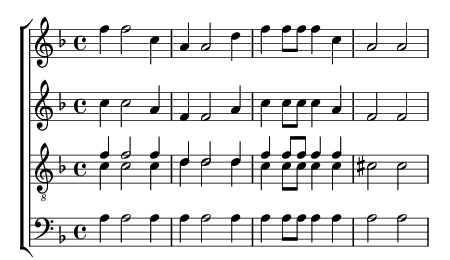
\includegraphics[scale=0.75]{lilypond/voices}
    \caption{Four part, five voice example}
    \label{fig:voicesExample}
  \end{center}
\end{figure}

\subsubsection{Ticks}

The ``tick\_value'' parameter is the most important parameter in VMF as this is the parameter which provides a time-duration value to each vector in the body. The tick value is the smallest rhythmic unit that can be represented in a given VMF file. This smallest unit is referred to as a ``tick''. The value which is assigned to this parameter expresses the fraction of a quarter note which is equivalent to a single tick. Table \ref{tab:tickValues} illustrates some common tick values.

\begin{table}[ht]
  \centering
  \begin{tabular}{ll}
  Tick Value & Equivalent Rhythmic Unit \\ \hline
  4          & 1 whole note             \\
  2          & 1 half note              \\
  1          & 1 quarter note           \\
  1/2        & 1 eighth note            \\
  1/3        & 1 triplet eighth note    \\
  1/4        & 1 sixteenth note        
  \end{tabular}
  \caption{Common Tick Values}
  \label{tab:tickValues}
\end{table}

\subsubsection{Time Signatures, Key Signatures, and Metronome}

The last header parameters of importance are ``time\_signature'', ``key\_signature'', and ``tempo''. These three parameters all have the same structure; a JSON object containing key-value pairs where the key is the offset from the begininning of the piece in ticks, and the value is the key signature, time signature or metronome marking at that position.

The value of a time signature item is formatted as a fraction (``upper value/lower value''), and the value of a tempo item is an integer representing beats per minute. The value of a key signature is represented as an integer indicating the number of sharps or flats which appear in a key signature (ex. ``4'' indicates four sharps, and ``-4'' indicates four flats). Table \ref{tab:keySignatures} provides a summary of the key signature encoding.

\begin{table}[ht]
  \centering
  \begin{tabular}{lll}
    Major Key & Minor Key & Encoding \\ \hline
    $C\sharp$   & $A\sharp$   & 7        \\
    $F\sharp$   & $D\sharp$   & 6        \\
    $B$         & $G\sharp$   & 5        \\
    $E$         & $C\sharp$   & 4        \\
    $A$         & $F\sharp$   & 3        \\
    $D$         & $B$         & 2        \\
    $G$         & $E$         & 1        \\
    $C$         & $A$         & 0        \\
    $F$         & $D$         & 1        \\
    $B\flat$    & $G$         & 2        \\
    $E\flat$    & $C$         & 3        \\
    $A\flat$    & $F$         & 4        \\
    $D\flat$    & $B\flat$    & 5        \\
    $G\flat$    & $E\flat$    & 6        \\
    $C\flat$    & $A\flat$    & 7        
  \end{tabular}
  \caption{Key Signature Encoding}
  \label{tab:keySignatures}
\end{table}

Now that each of the header paramters have been defined, in Figure \ref{fig:voicesHeader}, the appropriate header is displayed for the western music notation in Figure \ref{fig:voicesExample}

\begin{figure}
  \begin{center}
    \begin{Verbatim}[fontfamily=courier, xleftmargin=\parindent]
    {
      "header": {
        "tick_value": "1/2",
        "number_of_parts": 4,
        "number_of_voices": 5,
        "time_signature": {
            "0.0": "4/4"
        },
        "key_signature": {
            "0.0": -1
        },
        "tempo": {
          "0.0": 93
        }
      }
    }
    \end{Verbatim}
    \caption{Appropriate header for music in Figure \ref{fig:voicesExample}}
    \label{fig:voicesHeader}
  \end{center}
\end{figure}

\subsection{VMF Body}

\subsubsection{Arrangement of Arrays in Tick}

The body of a VMF file consists of a JSON array containing one or more JSON arrays. Each of these sub arrays represents a single tick in time where the duration of this tick is that which is defined in the header. Within each ``tick array'', there is one array for each voice which is identified in the header. If there are five voices in a score, then each tick array should have 5 sub arrays within it. The contents of these sub arrays is the data representing each voice's musical data at that instance in time. Figure \ref{fig:fiveVoiceTick} is an illustration of how the body would be structured for the first tick of the music of Figure \ref{fig:voicesExample}.

\begin{figure}
  \begin{center}
    \begin{Verbatim}[fontfamily=courier, xleftmargin=\parindent]
    {
      "body": [
        // This outer array is a single tick. Represents a
        // single instance in time.
        [
          // These inner arrays are the representation of each
          // voice's musical data at this instance in time.
          [1,-1,0,5,5,0],
          [1,-1,0,0,5,1],
          [1,-1,0,4,4,2],
          [1,-1,0,0,4,2],
          [1,-1,0,9,3,3]
        ],
        ...
      ]
    }
    \end{Verbatim}
    \caption{Body structure for the first tick of the music in Figure \ref{fig:voicesExample}}
    \label{fig:fiveVoiceTick}
  \end{center}
\end{figure}

\subsubsection{Time}

VMF requires that each tick looks the same in terms of number of voices and vector length. If Figure \ref{fig:fiveVoiceTick} were to be extended, each subsequent tick would have five sub arrays, each with six dimensions just like the first tick. One way to think of this structure is that each voice during a given tick is represented by a vector and each tick is represented by a matrix formed by the combined vectors of each part.

Since each tick represents the smallest rhythmic unit, in order to represent notes of a longer duration, an encoding is used in each vector to signify one of three possible states.

If a note is attacked in a given tick, the first dimension of the vector will 1. If a note is sustained from the previous tick (in order to elongate a note), the first dimension of the vector will be 2. If there is silence in this tick, the first dimension of the vector will be 0.

These three states are mutually exclusive and are summarized in Table \ref{tab:attackBits}.

\begin{table}[ht]
  \centering
  \begin{tabular}{ll}
  Attack Dimension & Interpretation \\ \hline
  0          & Rest             \\
  1          & Attack              \\
  2          & Sustain           \\
  \end{tabular}
  \caption{Interpretation of the Attack Dimension}
  \label{tab:attackBits}
\end{table}

A special case comes up when dealing with music where the time signature changes, either temporarily (tuplets), or for a longer period of time. In this case, the greatest common denominator of the two time systems will be used. For example, if a piece is in the 4/4 time signature (with a tick value of 1/2), and a triplet (with a tick value of 1/3) is encountered, a global tick value of 1/6 (1/2 * 1/3) will be used to accommodate both systems. An example of this scheme is illustrated in Figure \ref{fig:mixedMeterVMF} where the music contained in Figure \ref{fig:mixedMeterWestern} is encoded.

\begin{figure}
  \begin{center}
    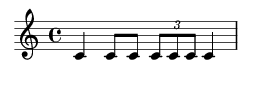
\includegraphics[scale=0.75]{lilypond/mixedMeter}
    \caption{Triplet in 4/4 Time}
    \label{fig:mixedMeterWestern}
  \end{center}
\end{figure}

\begin{figure}
  \begin{center}
    \begin{Verbatim}[fontfamily=courier, xleftmargin=\parindent]
    {
      "header": {
        "tick_value": "1/6",
        "number_of_parts": 1,
        "number_of_voices": 1,
        "time_signature": { "0.0": "4/4" },
        "key_signature": { "0.0": 0 },
        "tempo": { "0.0": 100 }
      },
      "body": [
        // Each beat is seperated by a line for clarity.
        [[1,-1,0,0,4,0]],
        [[2,-1,0,0,4,0]],
        [[2,-1,0,0,4,0]],
        [[2,-1,0,0,4,0]],
        [[2,-1,0,0,4,0]],
        [[2,-1,0,0,4,0]],

        [[1,-1,0,0,4,0]],
        [[2,-1,0,0,4,0]],
        [[2,-1,0,0,4,0]],
        [[1,-1,0,0,4,0]],
        [[2,-1,0,0,4,0]],
        [[2,-1,0,0,4,0]],

        [[1,-1,0,0,4,0]],
        [[2,-1,0,0,4,0]],
        [[1,-1,0,0,4,0]],
        [[2,-1,0,0,4,0]],
        [[1,-1,0,0,4,0]],
        [[2,-1,0,0,4,0]],

        [[1,-1,0,0,4,0]],
        [[2,-1,0,0,4,0]],
        [[2,-1,0,0,4,0]],
        [[2,-1,0,0,4,0]],
        [[2,-1,0,0,4,0]],
        [[2,-1,0,0,4,0]],
      ]
    }
    \end{Verbatim}
    \caption{VMF for Figure \ref{fig:mixedMeterWestern}}
    \label{fig:mixedMeterVMF}
  \end{center}
\end{figure}

This system is also extensible for cases where more than two systems are found together (ex. duple, triple, and n-tuple). In this case, the greatest common denominator satisfying all three systems will be used as it was in the previous example.

It must also be noted that when pickup measures are present, they are encoded as a full measure with the incomplete part padded with silence vectors.

\subsubsection{Pitch}

Now that the encoding system for rhythm has been established, the pitch encoding system is next to be discussed. In VMF, pitch information is divided into two parts, the pitch class and the octave. Starting from pitch class C to pitch class B, each pitch class is given an integer starting from 0. Table \ref{tab:pitchClassEncoding} provides a summary of this mapping. The octave part of a pitch is reporesented using the octave designations from the international pitch notation (ex. middle C is C4). As an example, the pitch for middle C in VMF would have 0 as the pitch class value and 4 as the octave value. Referring back to Figure \ref{fig:fiveVoiceTick}, the pitch class and octave dimensions can be seen used in conjunction.

\begin{table}[ht]
  \centering
  \begin{tabular}{ll}
  Pitch Class & VMF Encoding \\ \hline
  0           & $C$            \\
  1           & $C\sharp$, $D\flat$      \\
  2           & $D$            \\
  3           & $D\sharp$, $E\flat$      \\
  4           & $E$            \\
  5           & $F$            \\
  6           & $F\sharp$, $G\flat$      \\
  7           & $G$            \\
  8           & $G\sharp$, $A\flat$      \\
  9           & $A$            \\
  10          & $A\sharp$, $B\flat$      \\
  11          & $B$            
  \end{tabular}
  \caption{Pitch Class Encoding}
  \label{tab:pitchClassEncoding}
\end{table}

\subsubsection{Chords}

The encoding method for chords works just like it does for individual pitches, but the vector length is extended to accomodate the additional notes. Because in VMF each vector must have the same number of dimensions, during the encoding process, the largest chord in each voice must be determined so that each vector is the correct length. For example, if the largest chord has four notes as in Figure \ref{fig:chordsWestern}, the notes of each chord will be encoded in the vector from left to right ordered from lowest to highest pitch. If a vector has fewer notes then the largest chord, unused dimensions are padded with a value of -1 to indicate that this dimension is unused. An example of this encoding is seen in Figure \ref{fig:chordsVMF}.

\begin{figure}
  \begin{center}
    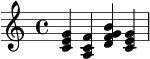
\includegraphics[scale=0.75]{lilypond/chords}
    \caption{Chord Progression}
    \label{fig:chordsWestern}
  \end{center}
\end{figure}

\begin{figure}
  \begin{center}
    \begin{Verbatim}[fontfamily=courier, xleftmargin=\parindent]
    {
      "body": [
        // Each beat is seperated by a line for clarity.
        [[1,-1,0,0,4,4,4,7,4,-1,-1,0]],
        [[1,-1,0,9,3,0,4,5,4,-1,-1,0]],
        [[1,-1,0,0,2,4,6,4,7,4,11,4,0]],
        [[1,-1,0,0,4,4,4,7,4,-1,-1,0]]
      ]
    }
    \end{Verbatim}
    \caption{VMF encoding of a Chord Progression}
    \label{fig:chordsVMF}
  \end{center}
\end{figure}

\subsubsection{Voices}

When a single part has multiple independent melodic voices, they are each encoded in their own vector within a tick as seen in \ref{fig:fiveVoiceTick} in the tenor part. In order to identify which part each voice belongs to, the last dimension in every vector is a part id. In this example, the soprano has an id of 0, the alto has an id of 1, both tenor voices have an id of 2, and the bass has an id of 3. With this system, voices can be regrouped if it is desired to reconstruct the encoded music in western notation.

\subsubsection{Dynamics and Articulation}

In VMF, dynamics and articulation each receive a dimension in a tick vector. The second dimension encodes dynamic and the third dimension encodes articulation. In both cases, the value of these dimensions can be determined using the following tables; Table \ref{tab:dynamicsMapping} for dynamics and Table \ref{tab:articulationsMapping} for articulations.

\begin{table}[ht]
  \centering
  \begin{tabular}{ll}
  Dynamic & VMF Encoding \\ \hline
  ppp      & -4 \\
  pp       & -3 \\
  p        & -2 \\
  mp       & -1 \\
  mf       & 1 \\
  f        & 2 \\
  ff       & 3 \\
  fff      & 4 \\
  \end{tabular}
  \caption{Dynamics Encoding}
  \label{tab:dynamicsMapping}
\end{table}

\begin{table}[ht]
  \centering
  \begin{tabular}{ll}
  Articulation & VMF Encoding \\ \hline
  No Articulation      & 0 \\
  Staccato             & 3 \\
  Staccatissimo        & 4 \\
  Strong Accent        & 5 \\
  Accent               & 6 \\
  Tenuto               & 7 \\
  \end{tabular}
  \caption{Articulation Encoding}
  \label{tab:articulationsMapping}
\end{table}

\subsubsection{Summary of Tick Definition}

As a summary of the definition of each positional dimention in a tick vector, Figure \ref{fig:vectorReference} is provided as a format structure key.

\begin{figure}
  \begin{center}
    \begin{Verbatim}[fontfamily=courier, xleftmargin=\parindent]
      [
        attack,
        dynamic,
        articulation, 
        pitch class 1, 
        octave 1, 
        pitch class 2, 
        octave 2, 
        ..., 
        part id
      ]
    \end{Verbatim}
    \caption{VMF Tick Legend}
    \label{fig:vectorReference}
  \end{center}
\end{figure}